
\documentclass{article}
\usepackage[utf8]{inputenc}
\usepackage{graphicx}
\usepackage{geometry}
\geometry{margin=0.5in}
\usepackage{amsmath}
\usepackage[table]{xcolor} % for color and colored shapes
\usepackage{amssymb}       % for symbols (optional)
\usepackage{fontspec} % Needed for emoji with XeLaTeX or LuaLaTeX
\usepackage{float}


\setlength{\parindent}{0pt} % Disable paragraph indentation
\setlength{\columnsep}{40pt} 

\newfontfamily\emojifont{Segoe UI Emoji}[Renderer=Harfbuzz]

%\newfontfamily\emojifont[Path=fonts/]{NotoColorEmoji-Regular.ttf}


\title{\textbf{Recommendo:} A Movie Recommendation WebApp}

\author{
    \textbf{ML Engineer} \\
    Davide Zorzetto \\
    \texttt{DAVIDE.ZORZETTO@studenti.units.it}
}

\date{\today}

\begin{document}

\twocolumn
\maketitle



\section*{ABSTRACT}

In this report, we present \textbf{Recommendo}, a machine learning-based web application for personalized movie recommendations. The site allows users to select five films they already enjoy and, through data-driven techniques, a recommendation engine computes movie similarities and generates personalized suggestions.


\section*{Introduction \& Problem Statement}
In a era  where users must choose between dozens of digital streaming platforms, they are often overwhelmed by the sheer volume of available films and series. This has led to a sort of paradox of choice,  where the abundance of possibilities brought onto users decision fatigue. 

Another key point is that, while there are tradition recommendation systems embedded directly into these services, they are not always transparent or personalized, particularly when users’ history is not present.

Our proposal, Recommendo, has been built with these challenges in mind: we allow users to select up to 10 (at least one) films they already like and then return tailored recommendations based on those choices. The core of our project is a data-driven, machine learning-powered recommendation pipeline.
As a machine learning engineer, my role involved designing and implementing models, testing their performance, and collaborating closely with the data engineer to maximize the effectiveness of the system.



% _______________________________________
\section*{Background}
The development of our project required several things: we need to find coordination between modern web development practices, software design methodologies and data-driven machine learning components. 

At the beginning of the project, we decided to adopt an Agile software development methodology. We broke down the work into weekly milestones with iterative improvements. 
Task tracking, collaboration, and version control were managed using GitHub Projects, which helped structure issues, pull requests, milestones, and more.

Each team member worked within their dedicated branch (e.g., \texttt{dev-architecture} for the SE, \texttt{dev-ml} for the MLE, \texttt{dev-app} for the SD, and \texttt{dev-data} for the DE). Merges into the main branch occurred only via reviewed pull requests, which were verified by the software engineer.

Initially, we considered Streamlit for the frontend, due to its easy integration with Python-based ML models. 
However, early in the development, the software developer brought up during a meeting that he felt it was too limited for the task at hand, and that he could do better if we transitioned to a more flexible stack: the Flask backend was built using Flask, to make the integration with python smoother while the frontend was built using HTML, CSS and JavaScript.

As the ML engineer, I had to select models that could operate effectively with minimal user input (1–10 film titles), deliver low-latency responses, and integrate seamlessly into a web-based pipeline. The models we considered and/or developed included:
\begin{itemize}
  \item k-NN on one-hot encoded features
  \item k-NN on embedding-based features (SBERT)
  \item Variational Autoencoder (VAE) on sentence embeddings — later discarded due to poor performance
\end{itemize}


We used a public Netflix dataset from Kaggle, which contains metadata such as title, cast, genre, description, and rating. Preprocessing was a critical step to prepare the data for both classical ML and embedding-based models.

The dataset management and preprocessing were handled by the data engineer, while their integration into the Flask backend required coordination with the software developer. The dataset we decided to use was a dataset containing Netflix’s Movies and TV-series, found on Kaggle.




% _______________________________________
\section*{Methodology/Approach}

\subsection*{Machine Learning Pipeline} 
The recommendation system was developed using a structured pipeline:

\begin{enumerate}
    \item \textbf{Data Preprocessing}: \\
        In collaboration with the data engineer, we handled heterogeneous features as follows:
        \begin{itemize}
            \item Categorical variables (\verb|director|, \verb|country|, \verb|cast|, \verb|listed_in|) were one-hot encoded
            \item High-cardinality one-hot features (e.g., \verb|cast|) were filtered to include only actors appearing in $\geq 5$ productions
            \item Text features (\verb|description|, \verb|listed_in|, \verb|cast|, \verb|title|) were embedded using Sentence-BERT
            \item \verb|duration| was converted to numerical format
            \item Numerical variables such as \verb|release_year| and \verb|rating| were normalized
            \item Non-informative variables (\verb|index|, \verb|date_added|) were dropped
            \item Observations with missing values (except in \\
            \verb|director|, \verb|cast|, and \verb|country|) were removed
    \end{itemize}


    \item \textbf{Feature Engineering}: \\
        We created two distinct feature spaces:
        \begin{itemize}
            \item \textit{Sparse Representation}: Traditional one-hot encoding of metadata
            \item \textit{Dense Representation}: SBERT embeddings \\ (\verb|all-MiniLM-L6-v2|) of textual descriptions
        \end{itemize}
        We assessed the quality of the embedded feature vectors using dimensionality reduction techniques such as \verb|t-SNE| and \verb|UMAP|.


    \item \textbf{Model Development}: \\
        We implemented and evaluated three approaches:
        \begin{itemize}
            \item \textit{KNN (One-Hot)}: Traditional k-Nearest Neighbors using mean squared error on sparse features
            \item \textit{KNN (Embedded)}, also named \verb|MLOVIE|: 
            A variant of KNN that uses cosine similarity in the SBERT embedding space for textual features and scores numerical features with $\frac{1}{\text{RMSE} + 1}$
            \item \textit{VAE}: Variational Autoencoder for latent space learning, later abandoned due to poor cluster separation in the latent space
        \end{itemize}

        In the KNN models, we introduced a hyperparameter to weight the relevance of different features. This improved performance by reducing the influence of less informative features (e.g., \verb|title|) and emphasizing more meaningful ones, such as movie genre.

    
    \item \textbf{Model Integration}: \\
        \begin{itemize}
            \item Designed a unified loading and prediction interface:
        \end{itemize}

        \begin{verbatim}
        def load(self):
            """Load necessary data"""

        def predict(IDX: list, k=5) -> np.ndarray:
            """Return top-k similar
            movie indices"""
        \end{verbatim}

        \begin{itemize}
            \item To suggest similar movies across all the user-selected films, the \verb|predict()| function first computes the closest movie for each input based on similarity score or distance. Then, it selects the movie with the highest overall score among those closest matches
            
            \item A similar \verb|fit()| interface was designed to compute the embeddings and store the resulting data

            \item Collaborated with the Data Engineer to fine-tune the model hyperparameters.
        \end{itemize}
     
\end{enumerate}


\subsection*{MLOps Implementation}
The machine learning lifecycle followed MLOps principles:
\begin{itemize}
    \item \textbf{Version Control}: Models, datasets, and preprocessing pipelines versioned in GitHub
    \item \textbf{Reproducibility}: Frozen dependencies via requirements.txt and model serialization
    \item \textbf{Testing}: Unit tests for embedding consistency and prediction stability
    \item \textbf{Monitoring}: Latency tracking during development (sub-second response achieved)
\end{itemize}




% _______________________________________
\section*{Results}

\subsection*{Performance Evaluation}
    Models were evaluated on four critical dimensions:
    \begin{table}[H]
    \centering
        \begin{tabular}{|l|c|c|}
            \hline
            \textbf{Metric}      & \raisebox{-0.3ex}{\emojifont 🟦} &   \raisebox{-0.3ex}{\emojifont 🟩}  \\
            \hline
            \hline
            Inference Speed (5 movies input) & $332  \ ms$              & $ 232 \ ms$              \\
            \hline
            Memory Footprint     & $ 82 \ MB$          & $ 62 \ MB$           \\
            \hline
            Cluster Coherence†   & low              & high               \\
            \hline
            Human Evaluation†    & medium           & high               \\
            \hline
            \hline
        \end{tabular}
        \caption{\footnotesize{ 
            {\emojifont 🟦}  KNN (One-Hot) 
            {\emojifont 🟩}  KNN (Embedded)  \\
            †Human evaluation: 4 users rated relevance (4 test users)} 
        }
    \end{table}
    
    The following plot shows how inference time increases as the number of input movies grows:

    \begin{figure}[h!]
        \centering
        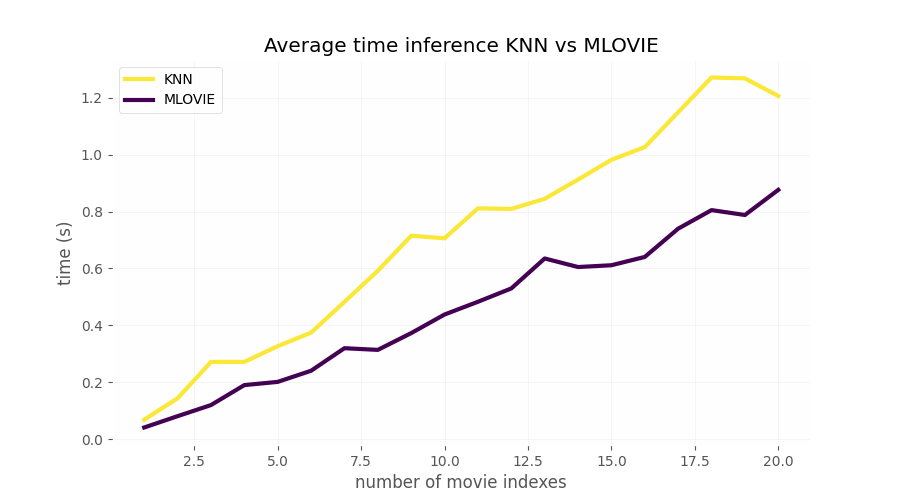
\includegraphics[width=0.5\textwidth]{time plot.png}
        \caption{inference time on both models}
        \label{fig:timeplot}
    \end{figure}


    The KNN (Embedded) model is consistently faster, and both models exhibit linear time growth. Although we set a limit of 5 movies for user input, the models can handle larger inputs without significant issues.

\subsection*{Key Findings}

The KNN (Embedded) model demonstrated superior performance across all evaluation metrics:
\begin{itemize}
    \item Achieved \textbf{$30\%$ faster inference} by avoiding high-dimensional computations
    \item Enabled semantic analysis of textual features such as \verb|description| and \verb|Title| 
    \item Produced more semantically coherent recommendations (validated via \verb|t-SNE| and \verb|UMAP| visualizations)
    \item Successfully integrated with backend through standardized interface
    
    \item Dimensionality of features:
    \begin{itemize}
        \item KNN (one-hot): $2356$ features (due to high cardinality from one-hot encoding)
        \item KNN (Embedded): $9$ features: $6$ SBERT embeddings (each with $384$ elements) plus $3$ normalized numerical features, resulting in $2307$ numerical values per observation
    \end{itemize}
\end{itemize}




\subsection*{System Outcomes}
\begin{itemize}
    \item Enabled for both models real-time suggestions ($<500 \ ms$ response time)

    \item Implemented a model-agnostic API supporting runtime switching:
    \begin{itemize}
        \item Designed a polymorphic interface enabling runtime model switching
        \item \textit{Implementation}: Standardized \texttt{predict()} method across models.
        \item \textit{Benefit}: Frontend can toggle between KNN and Embedded models via a dropdown menu.
    \end{itemize}Frontend can toggle between KNN/Embedded models via dropdown
\end{itemize}


    

  


% _______________________________________
\section*{Discussion \& Conclusion}

\subsection*{Technical Challenges}
Several challenges emerged during development:
\begin{itemize}
    \item \textbf{Heterogeneous Data}: TV shows and movies required different handling of duration
    \item \textbf{Semantic Gaps}: Plot descriptions often lacked thematic depth for accurate embeddings; more detailed descriptions would improve results in the KNN (Embedded) model
    \item \textbf{VAE Limitations}: Failed to learn meaningful latent representations from sparse features
    \item \textbf{Insufficient Metadata}: New movies without sufficient metadata remain challenging
\end{itemize}


\subsection*{System Limitations}
The current implementation has several constraints:
\begin{itemize}
    \item Static dataset (Netflix catalog as of 2021)
    \item Predictions are less accurate for movies with significant missing metadata (e.g. \verb |ratings|, \verb|listd_in|)
    \item No personalization beyond the initial seed movies
    \item Poor quality of movie descriptions
\end{itemize}


\subsection*{Conclusion}
The developed recommendation system successfully addresses the core requirement of generating personalized movie suggestions from minimal user input. The KNN approach using sentence embeddings proved optimal, balancing performance with recommendation quality. The modular design allows seamless incorporation of future improvements.



\subsection*{Future Enhancements}
\begin{itemize}
    \item Incorporate lightweight user feedback mechanism
    \item Incorporate external APIs for richer metadata:
    \begin{itemize}
        \item Richer descriptions could not only enable better movie recommendations but also allow search by user prompt descriptions
        \item User score ratings could provide valuable information to improve recommendations; currently, this information is used only on the UI and not by any model
    \end{itemize}
    \item Implement user feedback mechanism to improve recommendations
\end{itemize}

This project demonstrates that content-based filtering combined with modern NLP techniques provides effective recommendations while meeting the strict performance constraints required for web deployment. The MLOps approach ensured smooth integration between machine learning components and the production web environment.


\end{document}

